\subsection{Component interfaces}
Before showing the component interfaces, it is essential to show the class diagram of the model to be developed in order to
explain better what is next.

\begin{figure}[H]
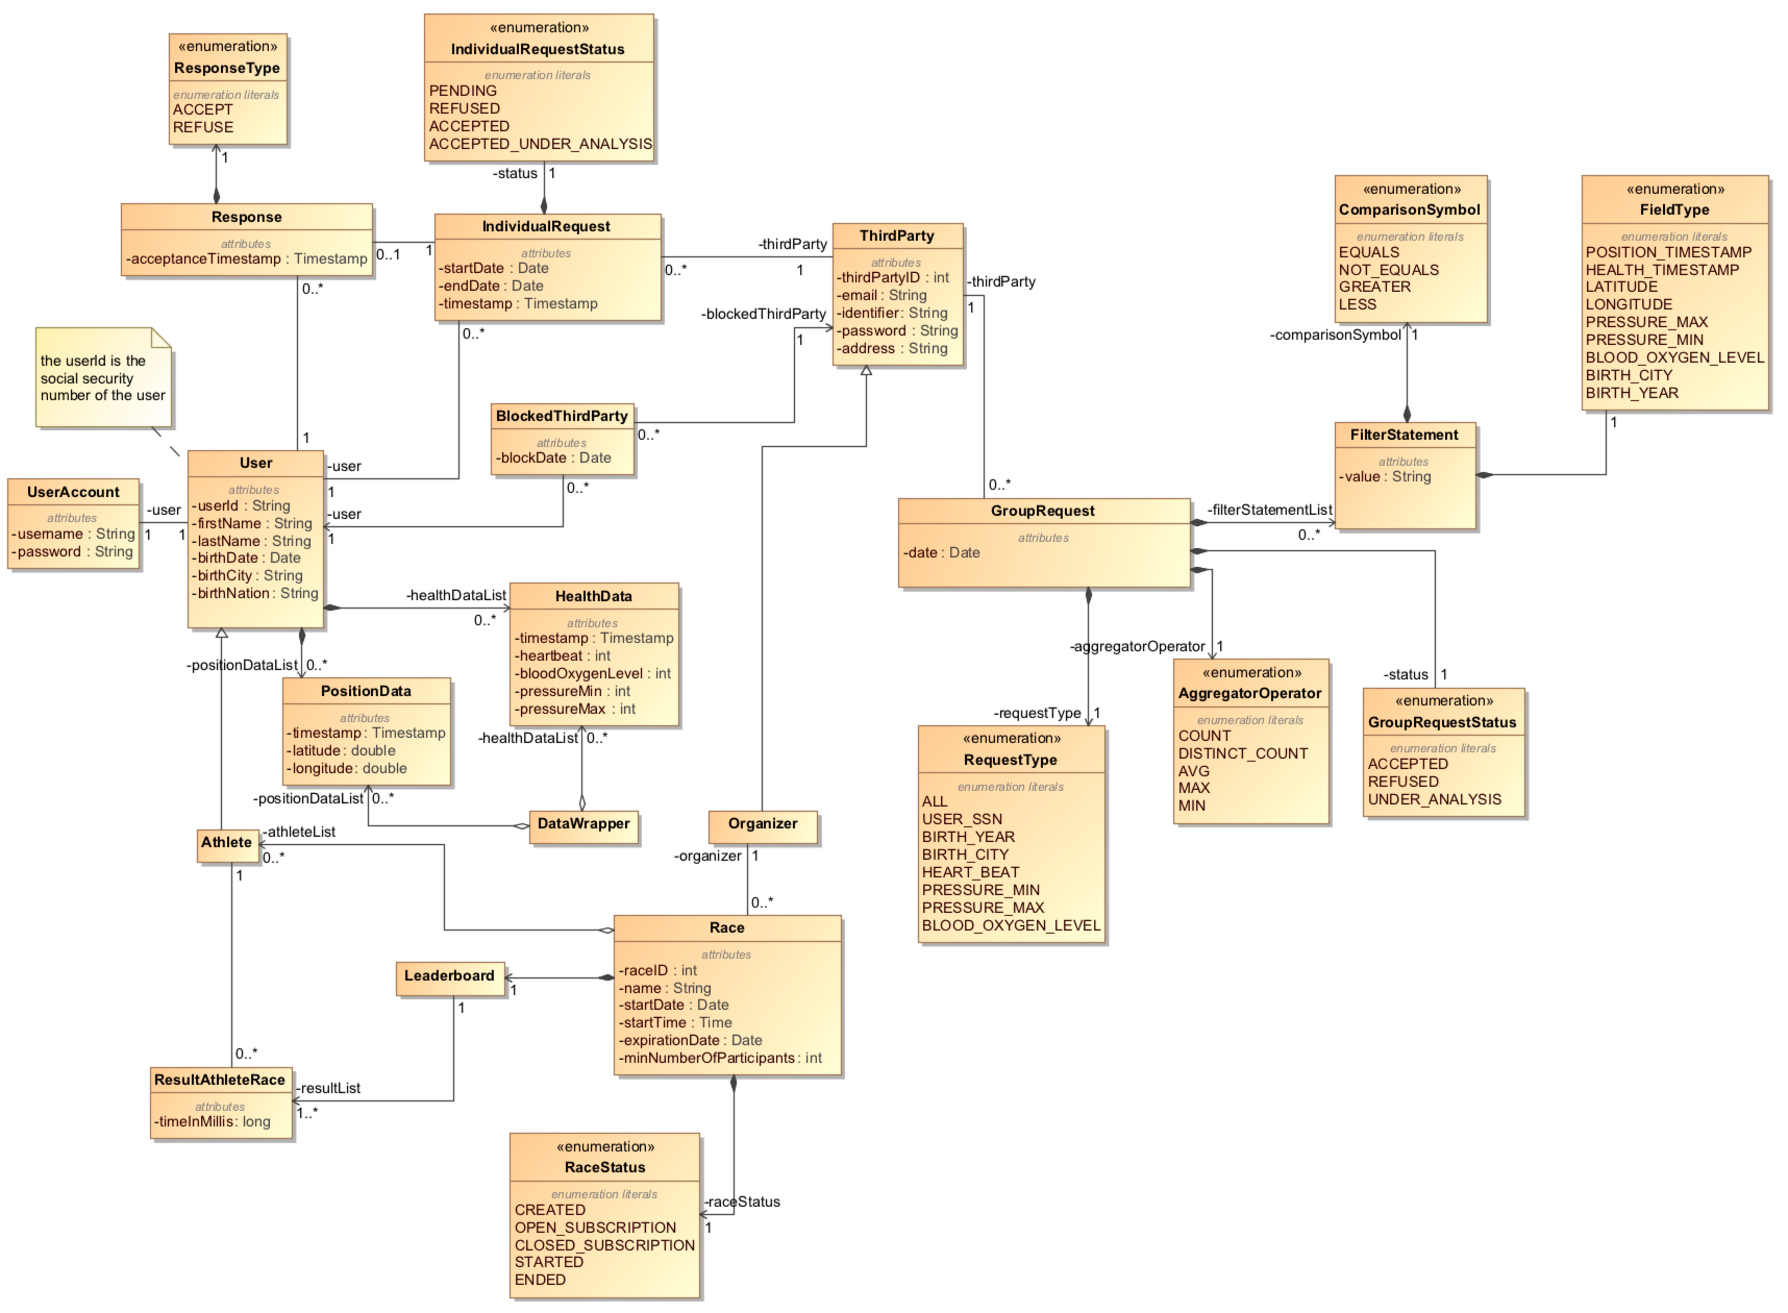
\includegraphics[width=\linewidth]{Images/classdiagram.pdf}
\caption{ Class diagram of the model }
\label{fig:classdiagram}
\end{figure}

Here follows the interfaces of the various components that are available. 
Note that interfaces of external components (e.g. DBMS's API, CallManagerInt, GPSInt, MapsAPI) are not present. 

\begin{figure}[H]
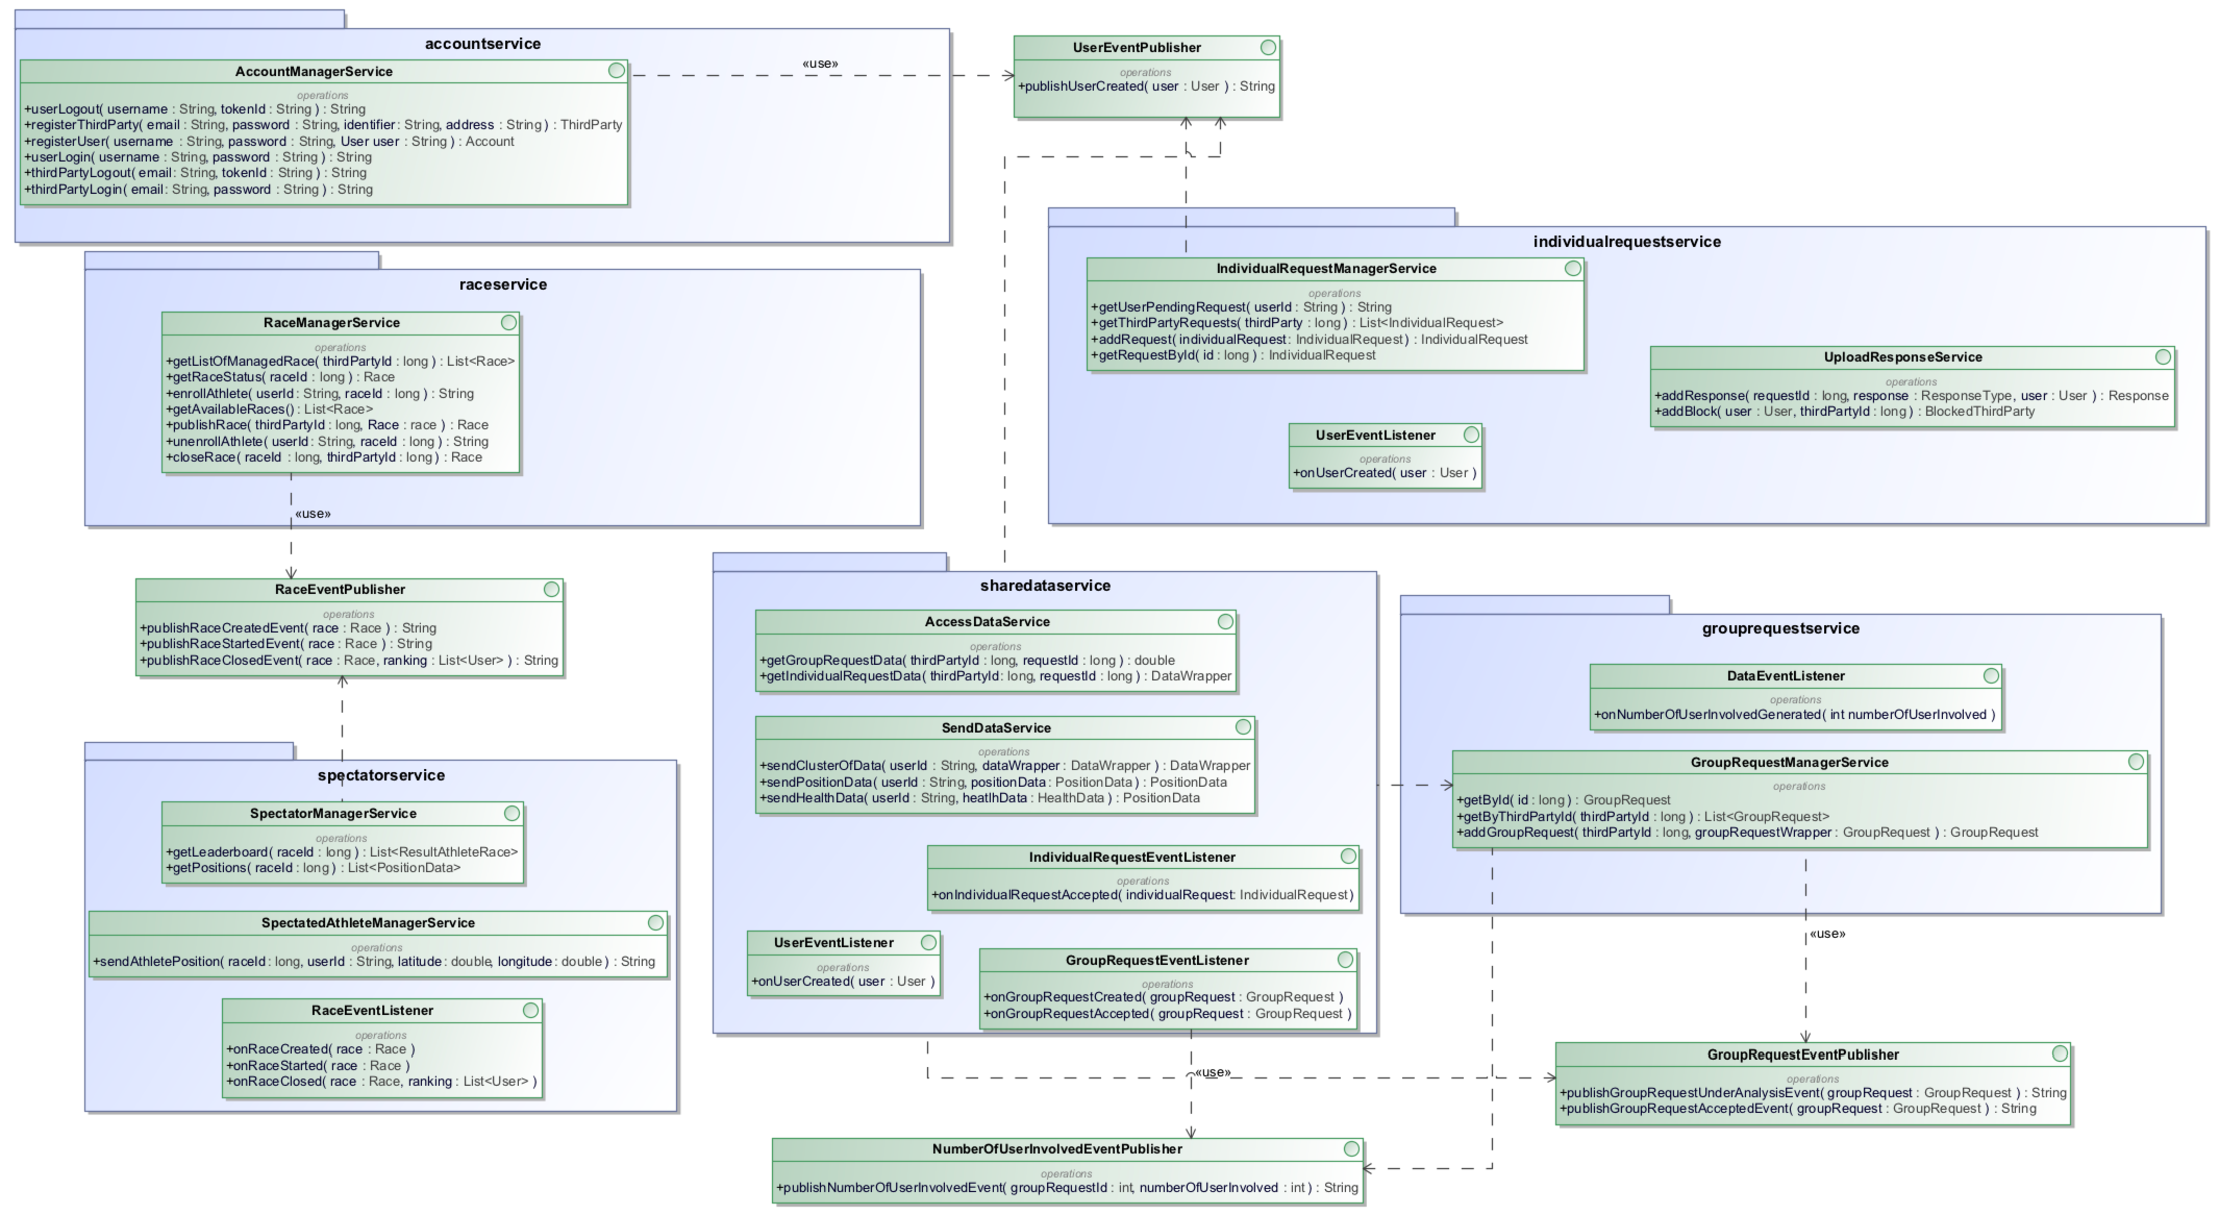
\includegraphics[width=\linewidth]{Images/componentinterfaces.pdf}
\caption{ Component interfaces }
\label{fig:componentinterface}
\end{figure}

In order to simplify the diagram, the API gateway has been excluded, but what it exposes is just the following: it provides a link for each
interface that is external w.r.t. the microservices block in figure \ref{fig:componentdiagram}. However, there is a little modification in the
parameters requested: indeed, the id of the client that is requesting the service (e.g. userID, thirdPartyID, athleteID) is substituted with
tokenID, in order to manage the authentication. This holds, clearly, with the exception of the registration and login feature, since a token 
is not available at this early stage of the user session. \\ 
A same reasoning is applied for what concerns the router: it just forwards the "translated" requests.